\casesection{Poiseuille flow with no-slip sidewalls\label{case:poiseuillenoslip}}


\paragraph*{Purpose}
The purpose of this validation case is to examine the performance of D-Flow FM for a plane Poiseuille flow simulation with a no-slip condition at the sidewalls. This no-slip condition inheres zero-velocities at the sidewalls. Poiseuille flow is pressure-induced flow in a long duct, in which case the flow is confined by two sidewalls. Poiseuille flow is distinguished from drag-induced flow such as Couette flow. Furthermore, it is assumed that there is laminar flow of an incompressible Newtonian fluid of dynamic viscosity $\mu$) induced by a constant positive pressure difference or pressure drop $\Delta p$ in a channel of length $L$ and width $B \ll L$. 


\paragraph*{Linked claims}
Claims that are related to the current test case are:
\begin{itemize}
\item \clrefnoh{cl:diffusionNoslip}
\end{itemize}


\paragraph*{Approach}
For this two-dimensional test case, $x$ and $y$ are defined as the longitudinal and lateral coordinates, respectively, with respective velocity components $u$ and $v$. The origin of the coordinate system is put at the center of the entrance of the channel. The flow is driven by a pressure gradient $\nabla p = (-P,0) = (-\rho g \Delta H / L,0)$ with $\Delta H$ the water level difference between the outflow boundary and inflow boundary, prescribing a flat bottom. The kinematic viscosity $\nu = \mu/\rho$ is used. Given the context of the shallow water equations, a uniform horizontal eddy viscosity $\nu_h$ is used instead. The velocities $u$ and $v$ can be shown to satify:
\begin{equation}
u(y) = \frac{g \Delta H}{8\nu L}\left(B^2 - 4y^2\right) \hspace{1cm} \textrm{and} \hspace{1cm} v = 0.
\end{equation}


\paragraph*{Model description}
A Cartesian grid consisting of $200 \times 20$ cells is established, covering a domain of sizes $L \times B$ equal to $10~\textrm{km} \times 1~\textrm{km}$. A flat bottom is used. The following flow settings are chosen:
\begin{itemize}
\item constant horizontal eddy viscosity $\nu_h = 0.1~\textrm{m}^2/\textrm{s}$,
\item water level drop $\Delta H = -1.0\cdot10^{-4}~\textrm{m}$.
\end{itemize}
Through these parameters, the analytical velocity profile is fully determined. The advection scheme nr. 3 (assigned as \texttt{Perot q(uio-u)}) is used. 



\paragraph*{Results}
First, the solution has to reach a steady state. To check if the steady state has been reached, the criterion $|\partial u / \partial t |_{\infty} < 10^{-10}~\textrm{m/s}^2$ is used. The computed velocity profile at the center of the domain is shown in comparison with the analytical solution in \Fref{fig:poiseuillenoslip}.

\begin{figure}[h!]
\begin{center}
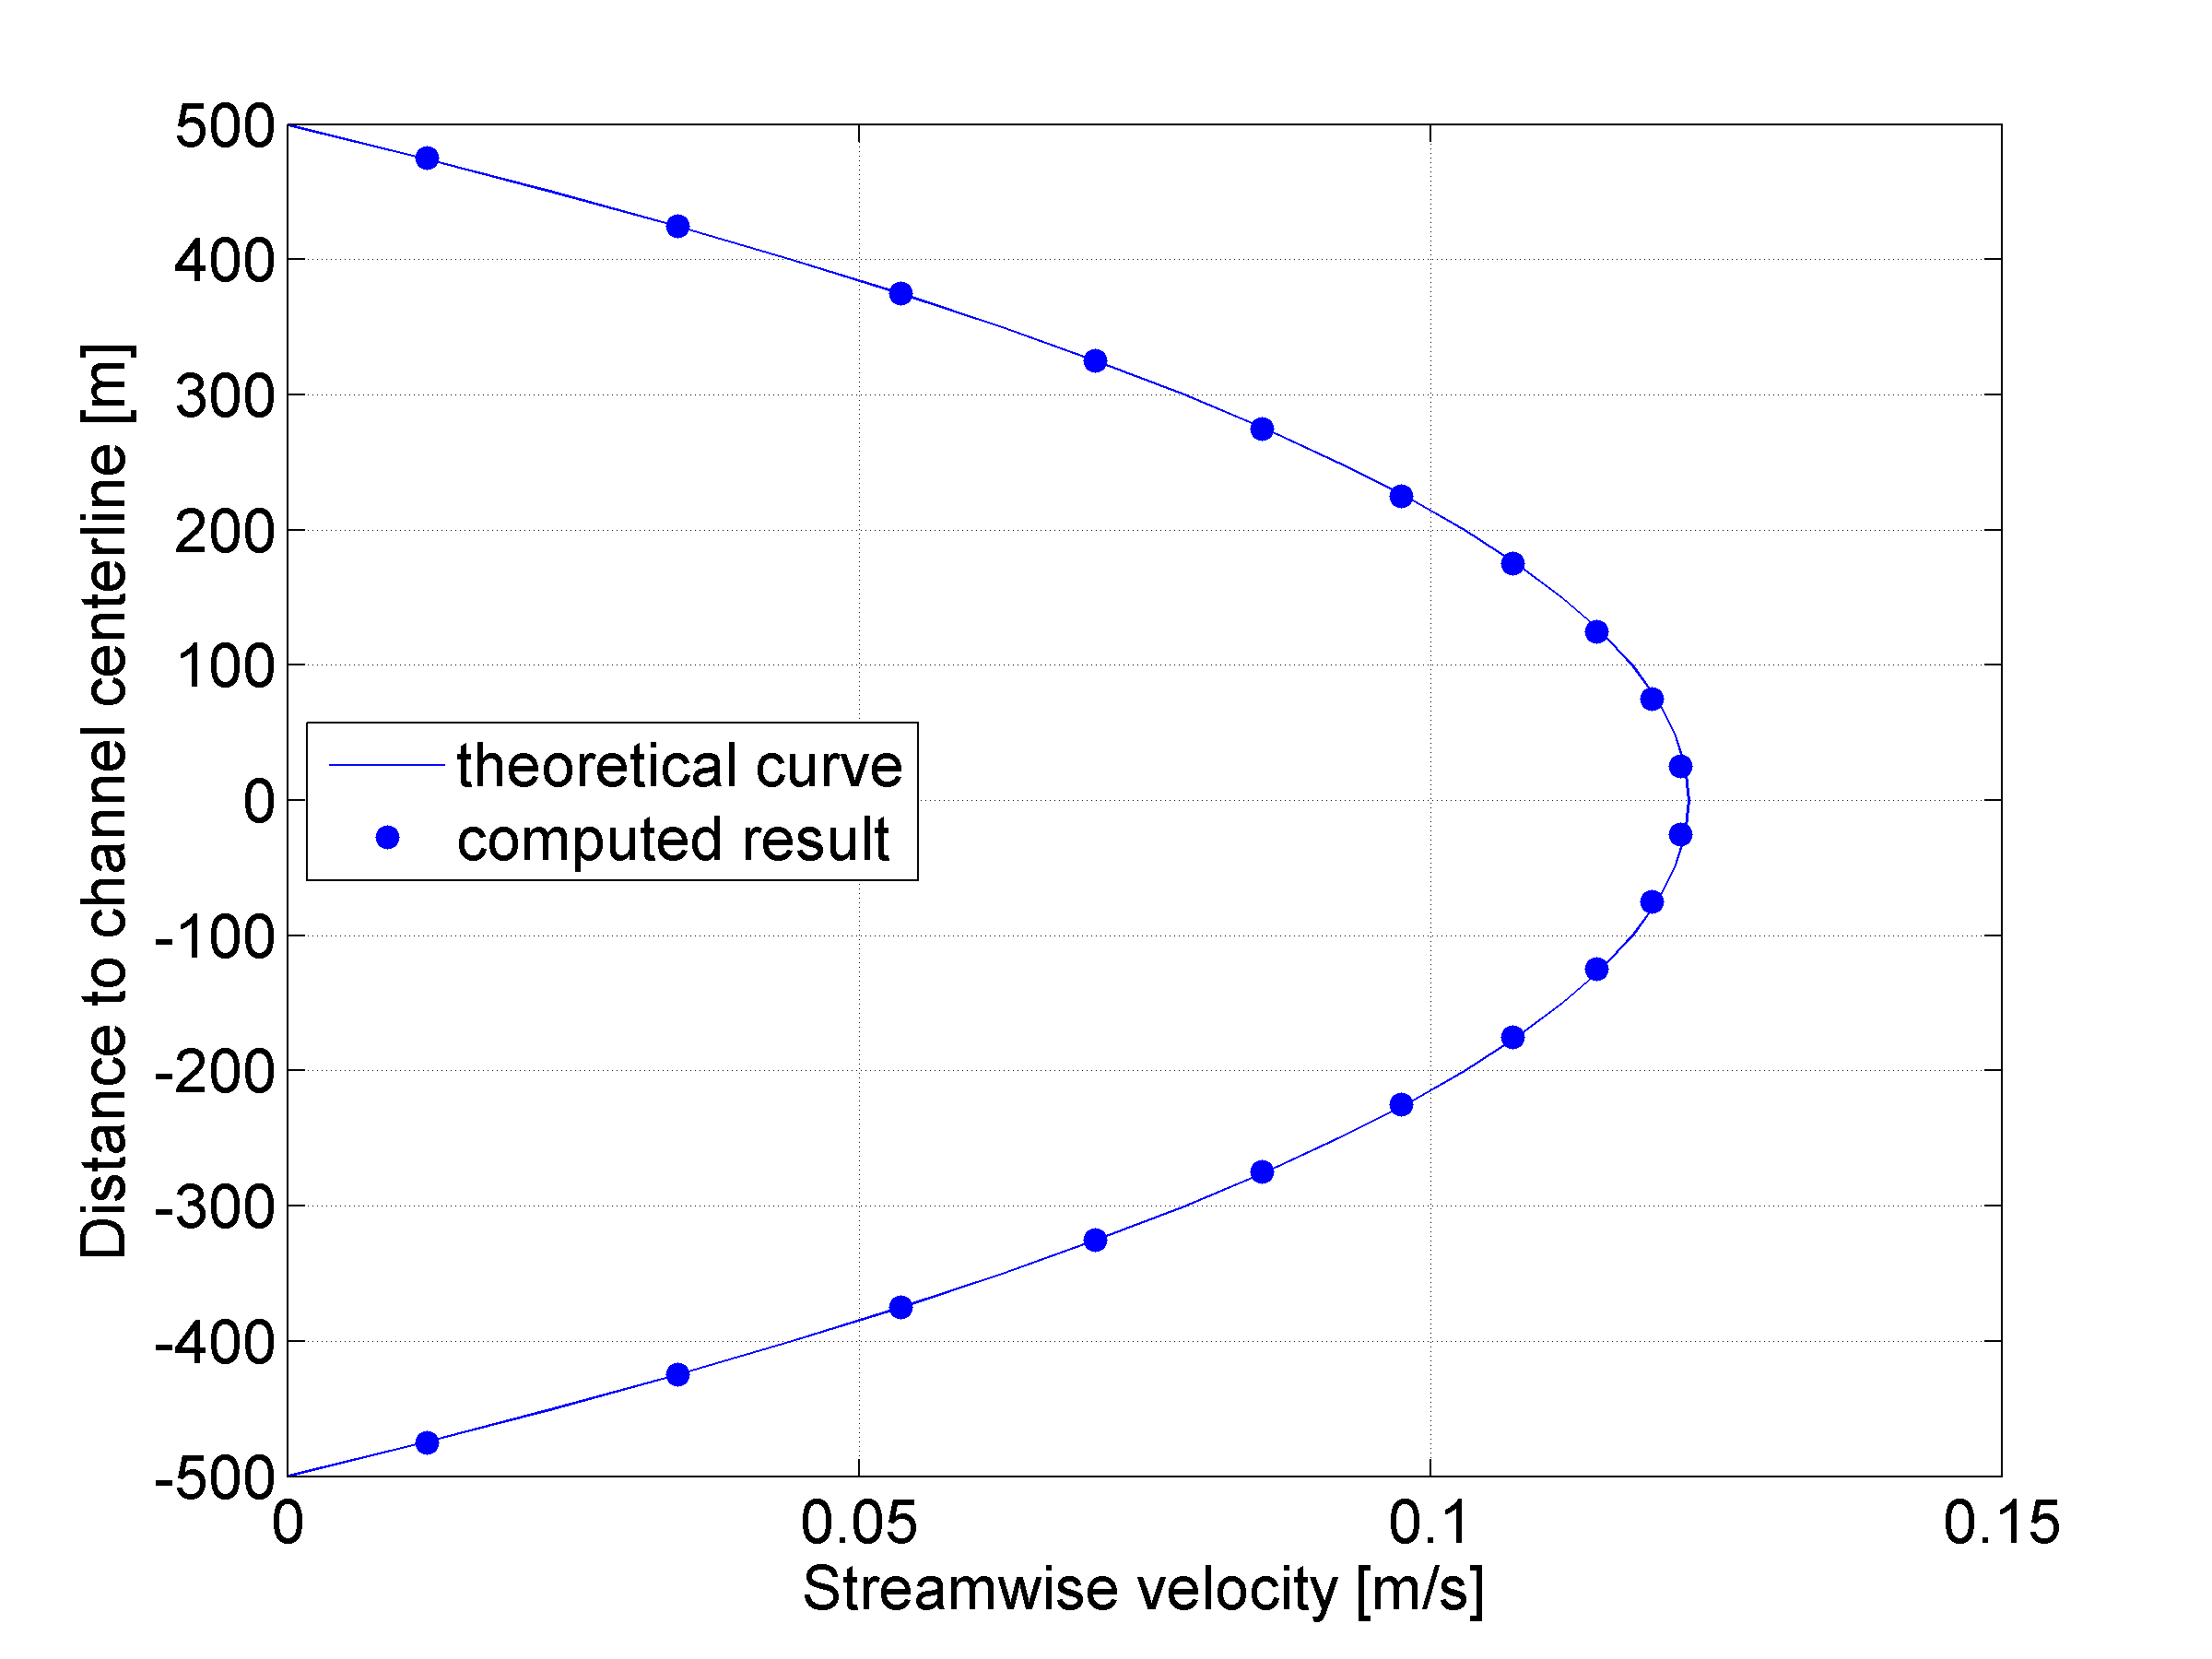
\includegraphics[width=0.65\columnwidth]{figures/poiseuillenoslip.png}
\end{center}\caption{Computed profile and analytical profile for the plane Poiseuille flow case with no-slip sidewalls. \label{fig:poiseuillenoslip}}
\end{figure}

The computed results tend to slightly underestimate the analytical results. The computed results near the centerline (not \emph{at} the centerline, due to staggering) differs -0.3507\% from its analytical counterpart. This issue is currently under investigation by Mart Borsboom. The maximum absolute lateral velocity is of the order of $10^{-8}~\textrm{m/s}$.




\paragraph*{Conclusion}
For plane Poisseuille flow with no-slip sidewalls, D-Flow FM approximates the analytical solution fairly well: the parabolic profile is reproduced and the maximum velocity is approximated within 1\% accuracy. The numerical results tend to underestimate the analytical results.



\paragraph*{Version}
This test has been carried out with version dflow-fm-x64-1.1.116.36629.


